% 第5章第2节：链与树上的动态规划（链上的接口表递推、树上的消息与后序、最优配置的回溯）。

\section{链与树上的动态规划}
\label{sec:graph-tree-dp}

本节只考虑一元项和成对项，并假定成对项组成的依赖图没有环。这时总成本为
\begin{equation}
F(\bm x)=\sum_{i\in V}\phi_i(x_i)+\sum_{\{u,v\}\in E}\phi_{u,v}(x_u,x_v),
\label{eq:graph-dp-pairwise-cost}
\end{equation}
其中$\mathcal G=(V,E)$是依赖图，$\phi_{u,v}(x_u,x_v)$与$\phi_{v,u}(x_v,x_u)$指同一个局部函数。没有一元项的变量可以取$\phi_i\equiv0$。本节从链开始，说明怎样把已经处理过的变量压缩成一张只依赖接口变量的表；再把单个前驱推广为多个子树，得到树上的消息；最后说明怎样从这些表中恢复一个最优配置。依赖图带环、或者局部函数读取三个以上变量的情形，留到下一节。

\subsection{链上的递推}

\paragraph{固定接口变量}
先看三个变量的链$1-2-3$，每个变量取三档$\{0,1,2\}$，总成本$F=\phi_{1,2}(x_1,x_2)+\phi_{2,3}(x_2,x_3)$。两张局部函数表按行列给出：
\[
\bigl[\phi_{1,2}(x_1,x_2)\bigr]=\begin{bmatrix}4&1&3\\2&3&5\\3&4&2\end{bmatrix},\qquad
\bigl[\phi_{2,3}(x_2,x_3)\bigr]=\begin{bmatrix}1&3&2\\4&3&5\\2&2&4\end{bmatrix},
\]
左表的行对应$x_1=0,1,2$、列对应$x_2=0,1,2$，右表的行对应$x_2$、列对应$x_3$。直接枚举要计算$3^3=27$个配置的成本。

注意$x_1$只出现在$\phi_{1,2}$中。若先把$x_2$固定为某个值，$x_1$的选择就不再影响$\phi_{2,3}$，只需在左表的这一列中取最小。对$x_2=0,1,2$分别取列最小值，得到一张只依赖$x_2$的表
\[
m_{1\to2}(x_2)=\min_{x_1}\phi_{1,2}(x_1,x_2)=(2,\,1,\,2),
\]
达到最小值的$x_1$依次为$1,0,2$。这张表概括了链左端的全部信息：无论右侧怎样取值，只要$x_2$给定，左端最好的做法和它的成本都已确定。接下来只需在$x_2,x_3$上求
\[
\min_{x_2,x_3}\bigl[m_{1\to2}(x_2)+\phi_{2,3}(x_2,x_3)\bigr].
\]
对$x_2=0,1,2$，括号内对$x_3$的最小值依次为$2+1=3$、$1+3=4$、$2+2=4$，所以最优成本为$3$，在$x_2=0,x_3=0$时达到，再查表得$x_1=1$。整个过程计算了$9+9=18$个候选值，而不是$27$个配置；更重要的是，链越长，节省越多。

\paragraph{为什么可以这样分步}
这一步依据有限集合上最小值的三条规则。设$y,z$分别在有限集合中取值，$h$、$g$取值于$\mathbb R\cup\{+\infty\}$，$c$与$y$无关，则
\begin{equation}
\min_{y,z}h(y,z)=\min_{z}\min_{y}h(y,z),\qquad
\min_{y}\bigl[g(y)+c\bigr]=\min_{y}g(y)+c,
\label{eq:graph-dp-min-rules}
\end{equation}
并且对取值于互不相交变量组$y_1,\ldots,y_k$的函数，$\min_{y_1,\ldots,y_k}\sum_{r}g_r(y_r)=\sum_r\min_{y_r}g_r(y_r)$。第一条成立，因为两边都是同一个有限数集中的最小元；第二条成立，因为加上同一个$c$不改变比较结果；第三条成立，因为各$y_r$可以分别取到各自的最小点，而任何选择都不会使某一项小于它的最小值。$c$或某项为$+\infty$时，按$+\infty$加任何数仍为$+\infty$的约定，三条规则依然成立。把第一、二条用于三变量链，$\phi_{2,3}$对$x_1$而言是固定加项，于是$\min_{x_1}$可以移到$\phi_{1,2}$上。

\paragraph{一般链的递推}
现在设链为$1-2-\cdots-n$，总成本含一元项$\phi_k(x_k)$和相邻成对项$\phi_{k-1,k}(x_{k-1},x_k)$。记$D_k(x_k)$为前$k$个变量在$x_k$固定时的最小部分成本，即对$x_1,\ldots,x_{k-1}$求最小值后的
\[
\sum_{i=1}^{k}\phi_i(x_i)+\sum_{i=2}^{k}\phi_{i-1,i}(x_{i-1},x_i).
\]
固定$x_k$以后，前$k-1$个变量与$x_k$之间只有$\phi_{k-1,k}$一项联系，按式~\eqref{eq:graph-dp-min-rules}先对$x_1,\ldots,x_{k-2}$求最小值，再对$x_{k-1}$求最小值，得到
\begin{equation}
\begin{gathered}
D_1(x_1)=\phi_1(x_1),\\
D_k(x_k)=\phi_k(x_k)+\min_{x_{k-1}\in\mathcal X_{k-1}}\bigl[D_{k-1}(x_{k-1})+\phi_{k-1,k}(x_{k-1},x_k)\bigr],\quad k=2,\ldots,n,
\end{gathered}
\label{eq:graph-dp-chain-recursion}
\end{equation}
整条链的最小成本为$\min_{x_n}D_n(x_n)$。对$k$归纳即得递推的正确性：$D_{k-1}$已经是前$k-1$个变量的最小部分成本，而$\phi_k(x_k)$与$x_{k-1}$无关，可以移出最小化。这种把问题按顺序拆开、为每个子问题保存最优值表并由前一张表算出后一张表的做法称为\term{动态规划}（dynamic programming）。

\begin{algorithm}[链上的最小成本递推]
\label{alg:graph-dp-chain}
输入：链上各变量的有限状态集合、一元项表和相邻成对项表。输出：最小成本和一个最优配置。
\begin{enumerate}
  \item 令$D_1(x_1)=\phi_1(x_1)$。
  \item 对$k=2,\ldots,n$和每个$x_k$，计算式~\eqref{eq:graph-dp-chain-recursion}方括号中的全部候选值，取最小值记为$D_k(x_k)$，并把达到最小值的$x_{k-1}$（并列时取编号最小者）记为$p_k(x_k)$。
  \item 取使$D_n$最小的$x_n$；再对$k=n,\ldots,2$令$x_{k-1}=p_k(x_k)$。
\end{enumerate}
\end{algorithm}

\paragraph{二值链的逐轮表}
取$n=4$的二值链，一元项为$\phi_1=(0,3)$、$\phi_2=(2,0)$、$\phi_3=(3,0)$、$\phi_4=(1,2)$，括号内依次是取$0$和取$1$的成本；相邻成对项在两端取值相同时为$0$，不同时为$2$。按式~\eqref{eq:graph-dp-chain-recursion}，$D_1=(0,3)$；$D_2(0)=2+\min(0+0,3+2)=2$，$D_2(1)=0+\min(0+2,3+0)=2$，故$D_2=(2,2)$；同理$D_3=(3+\min(2,4),\,0+\min(4,2))=(5,2)$，$D_4=(1+\min(5,4),\,2+\min(7,2))=(5,4)$。图~\ref{fig:graph-dp-chain-recursion}画出了每一轮的表和每个候选中被选中的前驱。最小成本为$\min D_4=4$，在$x_4=1$处达到。

\begin{figure}[!htb]
  \centering
  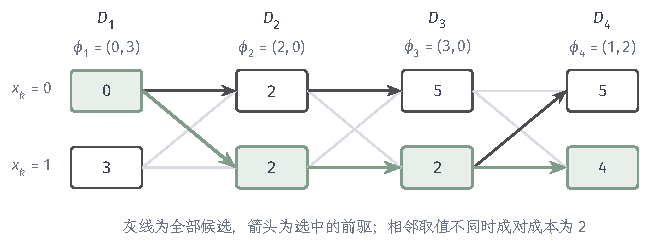
\includegraphics[width=109.587mm]{figures/01-basic-mathematics/04-graphs/tikz/c5-chain-recursion/figure.pdf}
  \caption{四变量二值链上的递推表。每列是一个变量，上下两格分别是$D_k(0)$与$D_k(1)$，列上方的小字为一元项。两列之间的灰色线表示全部候选，箭头从每个状态选中的前驱指向该状态，即回溯表$p_k$记录的选择。末列中$D_4(1)=4$最小，沿绿色箭头逆向读取得到最优配置$(0,1,1,1)$。逐点选取一元项最小的状态会得到$(0,1,1,0)$，成本为$5$。}
  \label{fig:graph-dp-chain-recursion}
\end{figure}

这个例子也说明了成对项的作用。若各变量只看自己的一元项，会选$(0,1,1,0)$：一元项合计为$1$，但两处取值变化要付$4$，总成本为$5$。递推得到的$(0,1,1,1)$在$x_4$上多付了$1$个单位的一元成本，却省掉了最后一处变化。

\paragraph{计算开销}
设每个变量至多有$q$个状态。每一轮要为$x_k$的每个状态比较至多$q$个候选，共至多$q^2$次候选计算，整条链约$nq^2$次。存储方面，每轮的$D_k$与回溯表$p_k$各至多$q$项，共约$2nq$项；若只要最优值而不恢复配置，任一时刻只需保留上一轮的表。与$q^n$次枚举相比，开销从指数降为线性于$n$。

\subsection{树上的递推}

\paragraph{从单个前驱到多个子树}
树没有链那样的天然顺序，但选定一个根$\rho$以后，每个非根顶点都有唯一的父点（第~\ref{sec:graph-trees-forests}节）。链上的$D_{k-1}$概括了$x_k$一侧的全部变量；在树上，一个顶点可能有多个子点，每个子点下面挂着一棵子树，需要分别概括后再合并。

对树的一条边$\{u,v\}$，删去它以后树分成两部分，记含$u$的那部分顶点集为$V_{u|v}$，称为$u$一侧。从$u$发往$v$的\term{消息}（message）是一张以$x_v$为索引的表，定义为
\begin{equation}
\begin{aligned}
m_{u\to v}(x_v)=\min_{x_u\in\mathcal X_u}\Bigl[&\phi_u(x_u)+\phi_{u,v}(x_u,x_v)\\
&+\sum_{r\in N(u)\setminus\{v\}}m_{r\to u}(x_u)\Bigr],
\end{aligned}
\label{eq:graph-dp-tree-message}
\end{equation}
其中$N(u)$是$u$在依赖图中的邻居集合。叶顶点只有一个邻居，求和为空，消息只由它自己的一元项和边上的成对项算出。下面的定理说明，这张表恰好概括了$u$一侧的全部成本。

\begin{theorem}[树上消息的含义]
\label{thm:graph-dp-tree-message}
设依赖图$\mathcal G=(V,E)$是有限树，总成本由式~\eqref{eq:graph-dp-pairwise-cost}给出。对任意边$\{u,v\}$，记$F_{u|v}$为$u$一侧的部分成本：$V_{u|v}$中各顶点的一元项、两端都在$V_{u|v}$中的成对项，再加上边$\{u,v\}$上的$\phi_{u,v}$。则对每个$x_v$，
\[
m_{u\to v}(x_v)=\min_{\bm x_{V_{u|v}}}F_{u|v}(\bm x_{V_{u|v}},x_v).
\]
进一步，对任意根$\rho$，$\min_{\bm x}F(\bm x)=\min_{x_\rho}\bigl[\phi_\rho(x_\rho)+\sum_{r\in N(\rho)}m_{r\to\rho}(x_\rho)\bigr]$。
\end{theorem}

\begin{proof}
对$|V_{u|v}|$归纳。删去$u$以后，$V_{u|v}\setminus\{u\}$按$u$的其他邻居$r\in N(u)\setminus\{v\}$分成互不相交的部分$V_{r|u}$。由树中路径的唯一性，不同部分之间没有边，否则会与$u$形成环。因此$F_{u|v}$可以拆成
\[
F_{u|v}=\phi_u(x_u)+\phi_{u,v}(x_u,x_v)+\sum_{r\in N(u)\setminus\{v\}}F_{r|u},
\]
其中每个$F_{r|u}$只依赖$x_u$与$\bm x_{V_{r|u}}$，并且每个局部项恰好出现在其中一处。固定$x_u$后，各$\bm x_{V_{r|u}}$是互不相交的变量组，由式~\eqref{eq:graph-dp-min-rules}后的第三条规则，对它们求最小值得到$\sum_r\min F_{r|u}$；由归纳假设，这个和等于$\sum_r m_{r\to u}(x_u)$。最后对$x_u$求最小值，就得到式~\eqref{eq:graph-dp-tree-message}。叶顶点是归纳的起点，此时求和为空，结论直接由定义得出。根处的等式用同样的拆分得到：$V\setminus\{\rho\}$按$\rho$的邻居分成互不相交的部分，每部分的最小成本是一条入消息。
\end{proof}

\paragraph{后序计算与分叉树算例}
式~\eqref{eq:graph-dp-tree-message}中，$u$发出消息前需要先收到来自其他邻居的消息。选定根后按后序处理顶点（先处理全部子点，再处理父点），每个顶点在收齐子点的消息后向父点发送一条消息，就满足了这个要求；最后在根处合并。图~\ref{fig:graph-dp-tree-messages}左半给出一个例子：树有边$\{1,3\},\allowbreak\{2,3\},\allowbreak\{3,4\},\allowbreak\{4,5\}$，以$3$为根；二值一元项为$\phi_1=(0,2)$、$\phi_2=(2,0)$、$\phi_3=(1,0)$、$\phi_4=(0,1)$、$\phi_5=(3,0)$；成对项在两端相同时为$0$，不同时分别为$1,1,2,1$（按上面边的顺序）。

后序为$1,2,5,4$。叶消息为$m_{1\to3}=(0,1)$，$m_{2\to3}=(1,0)$，$m_{5\to4}=(1,0)$，其中例如$m_{1\to3}(1)=\min(0+1,\,2+0)=1$。内部顶点$4$收到$m_{5\to4}$后向根发送
\[
\begin{aligned}
m_{4\to3}(x_3)&=\min_{x_4}\bigl[\phi_4(x_4)+\phi_{3,4}(x_3,x_4)+m_{5\to4}(x_4)\bigr]\\
&=\bigl(\min(0+0+1,\,1+2+0),\ \min(0+2+1,\,1+0+0)\bigr)=(1,1).
\end{aligned}
\]
根处合并一元项与三条入消息：$x_3=0$时为$1+0+1+1=3$，$x_3=1$时为$0+1+0+1=2$。因此最小总成本为$2$，根取$x_3=1$。整个计算只算了$4$条消息，每条消息比较$4$个候选，而枚举需要$2^5=32$个配置。

\begin{figure}[!htb]
  \centering
  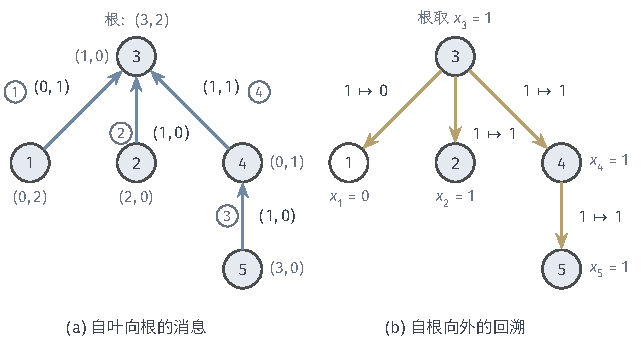
\includegraphics[width=108.514mm]{figures/01-basic-mathematics/04-graphs/tikz/c5-tree-messages/figure.pdf}
  \caption{分叉树上的消息与回溯。左：以$3$为根，按后序$1,2,5,4$发送消息；顶点旁的灰色二元组是一元项，箭头旁的二元组是消息表在接收端取$0$、$1$时的值，小圆圈中的序号是发送顺序；根合并后得到$(3,2)$。右：根取$x_3=1$后沿树向外查回溯表，黄色箭头旁的“$1\mapsto0$”表示父点取$1$时子点的最优选择为$0$；蓝色顶点取$1$，白色顶点取$0$，恢复的配置$(0,1,1,1,1)$成本为$2$。}
  \label{fig:graph-dp-tree-messages}
\end{figure}

\paragraph{每个顶点的最小成本表}
只求整体最优值时，一次自叶向根的计算已经足够。有时还需要知道每个顶点$v$取各个状态时整体能达到的最小成本，即$\min_{\bm x:\,x_v=s}F(\bm x)$。对根，这就是根处的合并结果；对其他顶点，还缺少来自父点一侧的消息。这时再按前序从根向叶发送一遍消息，同样使用式~\eqref{eq:graph-dp-tree-message}，然后在每个顶点合并全部入消息与一元项。仍以上例，从根发往$1$的消息为$m_{3\to1}=(2,1)$，于是$x_1$取$0$、$1$时的最小总成本为$(0+2,\,2+1)=(2,3)$，其最小值与整体最优值$2$一致。两遍计算共发送$2(n-1)$条消息；没有用到的方向不必计算。

\paragraph{计算开销}
每条消息对$x_v$的每个状态比较$x_u$的至多$q$个状态，每个候选要加上$|N(u)|$项，所以发出全部向上消息共需$O\bigl(\sum_u|N(u)|q^2\bigr)=O(nq^2)$次加法和比较，其中用到了树中$\sum_u|N(u)|=2(n-1)$。存储为$n-1$张消息表，每张至多$q$项。

\subsection{最优配置的回溯}

最优值只告诉我们最小成本是多少，并不直接给出达到它的配置。消息表经过了最小化，已经丢掉了“是哪一个$x_u$达到最小”的信息；若只保存最优值，事后只能重新枚举。解决办法是在计算每条消息时，为接收端的每个状态$x_v$同时记录达到最小值的$x_u$，组成一张\term{回溯表}$b_{u\to v}(x_v)$。并列最优时需要事先固定选择规则，本节约定取编号最小的状态。

\paragraph{从根向外读取}
回溯从根开始：取使根处合并值最小的$x_\rho$；然后按前序，对每个已确定取值的顶点$v$及其子点$u$，令$x_u=b_{u\to v}(x_v)$。由于每个子点只由父点的取值决定，这一过程沿树向外恰好给每个变量赋值一次。在图~\ref{fig:graph-dp-tree-messages}右半中，根取$x_3=1$；查表得$b_{1\to3}(1)=0$、$b_{2\to3}(1)=1$、$b_{4\to3}(1)=1$；再由$x_4=1$得$b_{5\to4}(1)=1$。恢复的配置为$(x_1,\ldots,x_5)=(0,1,1,1,1)$。

回溯得到的配置确实达到最优值。对子树大小归纳可知：若$x_v$已经确定，按回溯表给$u$一侧赋值后，$u$一侧的部分成本$F_{u|v}$恰好等于$m_{u\to v}(x_v)$，因为每一步选的$x_u$都达到式~\eqref{eq:graph-dp-tree-message}中的最小值，而子树内部又由归纳假设达到各条入消息的值。在根处合并后，总成本就等于根处的最小合并值。图~\ref{fig:graph-dp-chain-recursion}中的绿色箭头是链上的同一过程。

\paragraph{结果核对与不可行情形}
把恢复的配置代回全部原始局部项，可以独立核对结果。上例中一元项依次为$0,0,0,1,0$，合计$1$；成对项中只有边$\{1,3\}$两端不同，贡献$1$；总成本为$2$，与根处的值一致，而且每个局部项只计了一次。这样的核对不依赖消息计算本身，能发现表格或下标上的错误。

若根处的最小合并值为$+\infty$，说明每个配置都被某个局部项禁止，问题没有可行配置。这时应直接报告不可行，而不是把回溯得到的配置当作最优解输出，因为在全为$+\infty$的表中任何选择都“达到”最小值。另外，回溯表只恢复一个最优配置；若要列出全部并列最优的配置，需要在每个状态记录全部最优选择，而这类配置的数目本身可能随$n$指数增长。
